Die hier besprochenen Grundlagen gehen nicht in eine Tiefe, um alle evtl. Fragen zu klären. Jedes einzelne Gebiet könnte eine Arbeit füllen. Stattdessen sollen lediglich einen kleinen Einblick geben.
\section{Künstliche Intelligenz}
Die Grafik \ref{img:classification_of_terms} soll die Einordnung von LLMs im Bereich der künstlichen Intelligenz zeigen.
\begin{figure}[!ht]
	\includegraphics[width=0.8\textwidth]{content/chapter_basics/images/einordnung_bezeichnungen.eps}
	\centering
	\caption{Einordnung LLMs}
	\label{img:classification_of_terms}
\end{figure}

In den folgenden Kapiteln werden die wichtigsten Technologien und Begriffe erläutert.\vspace{0.2cm}

Eine explizite Definition für künstliche Intelligenz ist zurzeit noch nicht erfolgt. Geschuldet ist diese Tatsache, da der Begriff Intelligenz nicht eindeutig definiert ist. Somit finden sich viele Versuche eine Definition für künstliche Intelligenz herzuleiten. In dieser Arbeit wird die Definition aus \cite[6 ff.]{definition_ki2019} verwendet.

\epigraph[text indent=0.5cm]{
	Systeme der künstlichen Intelligenz (KI-Systeme) sind vom Menschen entwickelte Softwaresysteme (und gegebenenfalls auch Hardwaresysteme)3, die in Bezug auf ein komplexes Ziel auf physischer oder digitaler Ebene handeln, indem sie ihre Umgebung durch Datenerfassung wahrnehmen, die gesammelten strukturierten oder unstrukturierten Daten interpretieren, Schlussfolgerungen daraus ziehen oder die aus diesen Daten abgeleiteten Informationen verarbeiten, und über das bestmögliche Handeln zur Erreichung des vorgegebenen Ziels entscheiden. KI-Systeme können entweder symbolische Regeln verwenden oder ein numerisches Modell erlernen, und sind auch in der Lage, die Auswirkungen ihrer früheren Handlungen auf die Umgebung zu analysieren und ihr Verhalten entsprechend anzupassen.
}

(\href{https://www.bitkom.org/sites/main/files/file/import/171012-KI-Gipfelpapier-online.pdf}{Wirtschaftliche Bedeutung ...}, 26 ff.).

\subsection{Historisches}
% aus: https://www.perplexity.ai/page/a-historical-overview-of-ai-wi-A8daV1D9Qr2STQ6tgLEOtg

An dieser Stelle eine kleine historische Exkursion in der Entwicklung der künstlichen Intelligenz.\vspace{0.2cm}

\begin{figure}[!ht]
	\includegraphics[width=0.8\textwidth]{content/chapter_basics/images/ai-winter-cycles.jpg}
	\centering
	\caption{KI Winterzyklen}
	\label{img:ai_winter_cycles}
\end{figure}

\textbf{1966: Rückschläge bei der maschinellen Übersetzung}\vspace{0.2cm}

\textbf{1969: Auswirkungen der Perzeptron-Kritik}\vspace{0.2cm}

\textbf{1971-75: Die Finanzierungsherausforderungen der DARPA}\vspace{0.2cm}

\textbf{1973: Der Fallout des Lighthill-Berichts}\vspace{0.2cm}

\textbf{1973-74: Kürzung der DARPA-Mittel}\vspace{0.2cm}

\textbf{1987: Zusammenbruch der LISP-Maschine}\vspace{0.2cm}

\textbf{1988: Kürzungen bei der strategischen Datenverarbeitung}\vspace{0.2cm}

\textbf{1990er Jahre: Niedergang von Expertensystemen}\vspace{0.2cm}

\textbf{1990er Jahre: Ende des Projekts der fünften Generation}\vspace{0.2cm}

\textbf{KI-Frühling des frühen 21. Jahrhunderts}\vspace{0.2cm}



\subsection{Maschinelles Lernen}
Das Gebiet um maschinelles Lernen (eng. Machine Learning) ist ein Teilgebiet der Künstlichen Intelligenz. Für das maschinelle Lernen wird in dieser Arbeit die allgemein gültige Definition nach Tom M. Mitchell verwendet.\vspace{0.2cm}

\epigraph[
author={Mitchell, Tom M},
source={Machine Learning},
translation={Ein Computerprogramm lernt aus Erfahrung E in Bezug auf eine Klasse von Aufgaben T und ein Leistungsmaß P, wenn sich seine Leistung bei Aufgaben in T, gemessen an P, mit der Erfahrung E verbessert.}
]{
	A computer programm is said to learn from experience E with respekt to some class of tasks T and performance measure P, if its performance at tasks in T, as measured by P, improves with experience E.
}

Bei dieser Definition ist,\\
\textbf{E} die \textbf{Erfahrung}, die Daten aus denen das System lernt,\\
\textbf{T} beschreibt die \textbf{Aufgabe}, die das System erledigen soll und\\
\textbf{P} ist die \textbf{Leistungskennzahl} an dem der Erfolg des Systems die Aufgabe zu lösen gemessen wird.\vspace{0.2cm}
%Da es mehrere Definitionen maschinellen Lernens gibt definieren WITTEN ET AL. (2001:6) eine operationale Definition von Lernen: „Etwas lernt, wenn es sein Verhalten so ändert, dass es in Zukunft eine bessere Leistung aufweist.“

Maschinelles Lernen (\acrshort{ML}) und Künstliche Intelligenz (\acrshort{KI}) sind nicht wirklich in der Lage selbstständig zu lernen oder denken, sie imitieren dies lediglich nach. Das maschinelle Lernen ist aber wohl in der Lage komplexe Muster und Funktionen in großen Datenmengen zu erkennen. Durch die Unfähigkeit zu lernen kann KI keine neuen Inhalte schaffen.\vspace{0.3cm}

Es ist auch egal wie gut die Modelle trainiert werden, eine 100\% Fehlerfreiheit gibt es nicht. Für die Praxis bedeutet dies, die Ausgaben von Modellen müssen durch Menschen immer wieder evaluiert werden, um dessen Richtigkeit sicherzustellen. Zudem sollten keine Modelle verwendet werden, wenn die Lösung eines Problems durch einen konkreten Algorithmus erfolgen kann. Hier können die Ergebnisse nachvollzogen werden und sind für den Menschen besser zu verstehen.\vspace{0.2cm}

\begin{figure}[!ht]
	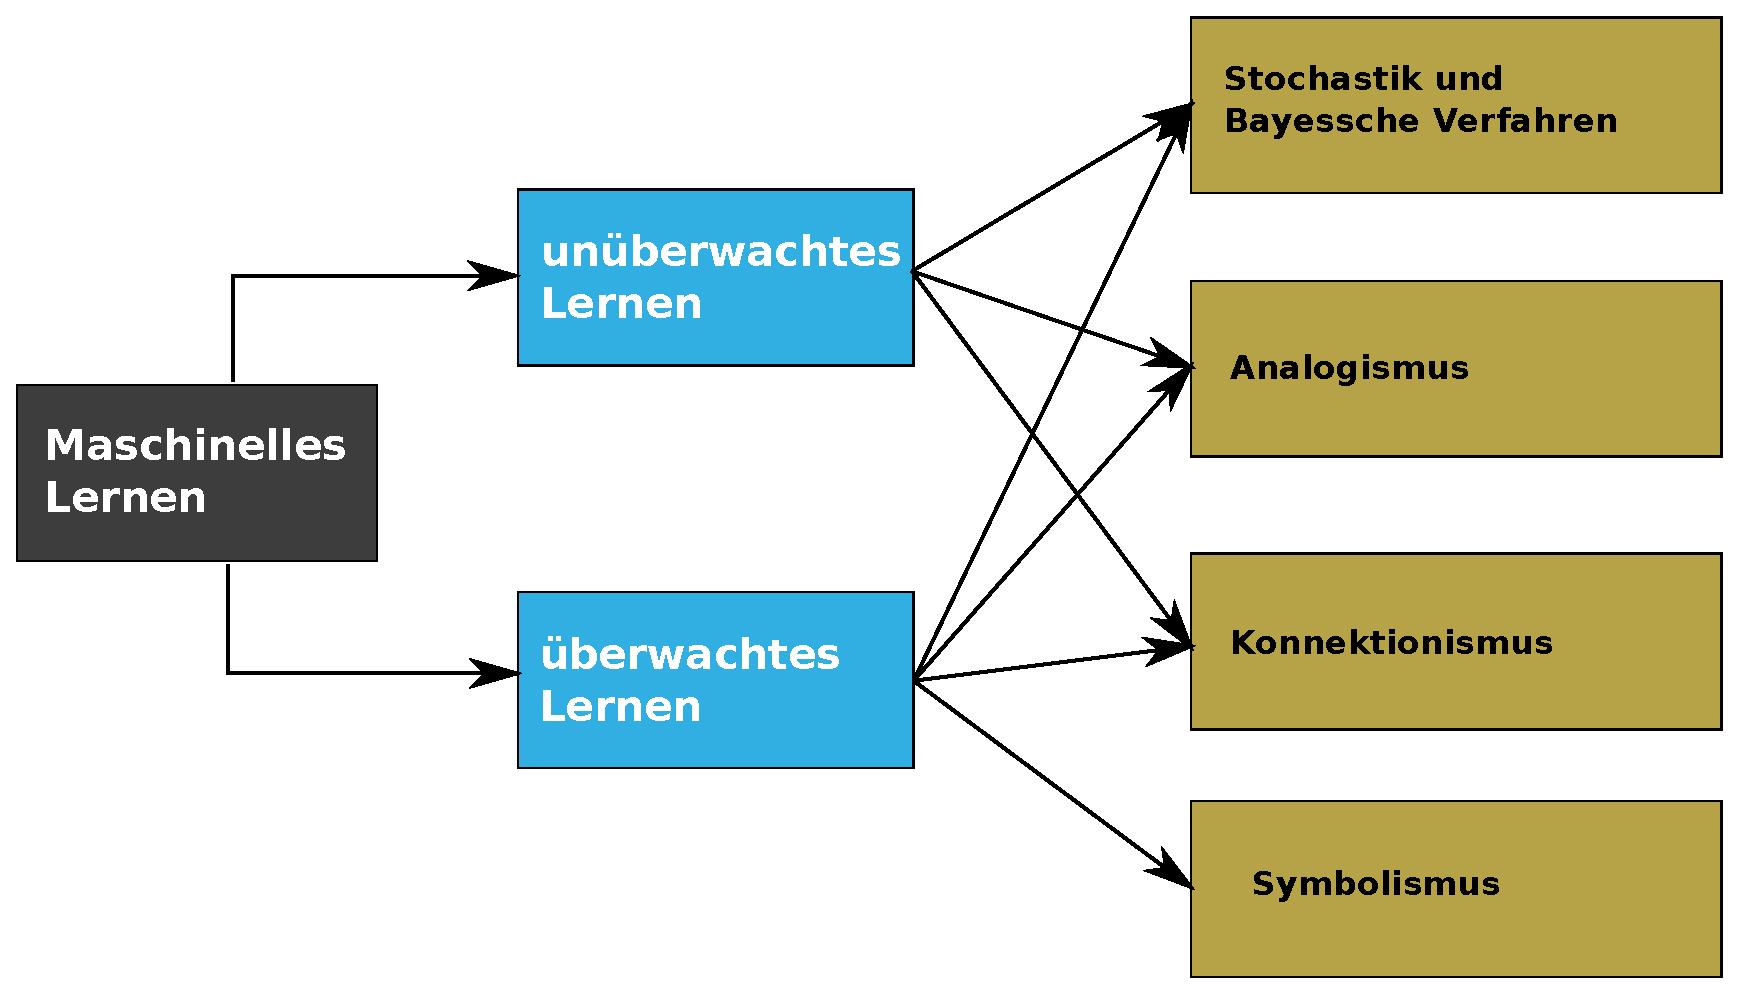
\includegraphics[width=0.8\textwidth]{content/chapter_basics/images/learning_paradigmen_ml_v2.eps}
	\centering
	\caption{Lernparadigmen des maschinellen Lernens}
	\label{img:learning_paradigms_of_ml}
\end{figure}


\subsection{Lernparadigmen des ML}
Das maschinelle Lernen wird in zwei wichtige Formen der Lernparadigmen unterteilt. Dem überwachten und dem unüberwachten Lernen. Abbildung \ref{img:learning_paradigms_of_ml} zeigt die wichtigsten Lernparadigmen des maschinellen Lernens.

\subsubsection{Überwachtes Lernen}
Bei überwachten Lernen sind für die Eingaben der Trainingsdaten dazugehörige Ausgaben (Labels) definiert. Das Ziel ist es eine Funktion zu trainieren um künftige Eingaben korrekt klassifizieren oder vorhersagen zu können.

\subsubsection{Unüberwachtes Lernen}
Bei unüberwachten Lernen sind die gelabelten Ausgaben nicht vorhanden. Hierbei wird beispielsweise durch Clustering oder Dimensionsreduktion versucht Muster und Strukturen zu erkennen.


\subsection{Theoretische Grundlagen}
In den folgenden Kapiteln werden vier wichtige Konzepte zum maschinellen Lernen besprochen. 

\subsubsection{Stochastik und Bayessche Verfahren}
Als Teilgebiet der Mathematik befasst sich die Stochastik mit Wahrscheinlichkeiten und zufälligen Prozessen. Auf dem Gebiet des maschinellen Lernens werden mithilfe der Stochastik Prognosen erstellt.\vspace{0.2cm}

Bei den Bayesschen Verfahren handelt es sich um stochastische Methoden, die auf dem Bayes-Theorem basieren. Hierbei werden neue Daten berücksichtigt, um die Wahrscheinlichkeit zu aktualisieren.\vspace{0.2cm}

Beide Methoden finden im überwachten und unüberwachtes Lernen Anwendung.

\subsubsection{Analogismus}
Dieser Lernansatz sucht nach Ähnlichkeiten in den Daten. Er basiert auf der Annahme, dass ähnliche Daten ähnliche Vorhersagen oder Klassifizierungen besitzen. Dieses Modell lernt, indem neue Daten mit bekannten vergleicht und nach ähnlichen Strukturen und Mustern sucht. Ein bekanntes Verfahren für diesen Lernansatz ist der k-Nearest Neighbors (\acrshort{k-NN}).\vspace{0.2cm}

Der Analogismus wird im überwachten Lernen als auch im unüberwachten Lernen angewandt, um Muster und Strukturen zuerkennen.

\subsubsection{Konnektionismus}
Der Lernansatz des Konnektionismus beruht auf kleine Einheiten die miteinander verbunden sind. Diese werden als Neuronen bezeichnet, die den Nervenzellen von Organismen nachempfunden sind. Die Künstlichen neuronalen Netze sind die bekanntesten Vertreter auf denen auch Deep Learning Modelle basieren.\vspace{0.2cm}

Auch dieser Lernansatz wird im unüberwachten und überwachten Lernen angewandt.

\subsubsection{Symbolismus}
Anders als beim Konnektionismus arbeiten die Einheiten beim Symbolismus mit explizite formale Regeln und Symbole, um das Wissen darzustellen. Der Symbolismus ist weniger flexible im Umgang mit unvollständigen Datensätzen und Unsicherheiten. Daher hat dieser Lernansatz weniger Relevanz als der Konnektionismus.\vspace{0.2cm}

Dieser Lernansatz findet im überwachten Lernen Anwendung, als Beispiel sind hier Entscheidungsbäume zu nennen.


\subsection{Neuronale Netze}
KNN

\subsubsection{Neuronen im neuronalen Netz}
Neuronen

\subsubsection{Arten der neuronalen Netzen}
KNN Arten

\subsubsection{Lernprozess im neuronalen Netz / Training}
Training

\subsection{Deep Learning}
DL

\subsection{Natural Language Processing}
NPL

\section{Large Language Model}
Large Language Model

\subsection{Grundlagen}
Grundlagen

\subsubsection{Tokenisierung}
Token

\subsubsection{Embedding}
Embedding

\subsubsection{Vorhersage}
Transformer

\subsubsection{Dekodierung}
Dekodierung

\subsection{Historie der LLM}
Historie

%\subsection{Weitere Begriffe bei LLMs}
%LLMs

%\subsubsection{Halluzinationen}

\section{Orchestrierung von LLMs}
Orchestrierung

\section{Multi-Agenten-Systeme}
Multi-Agent-System


%----------------------------------------------------------------

\section{Prompt Engineering}
Prompt Engineering optimiert die Antworten große Sprachmodelle, ohne Parameter, wie Bias und Gewichte des Models ändern zu müssen. Dieser Bereich hat in den letzten Jahren enorm an Bedeutung gewonnen und sich zu einer eigenen Disziplin im Bereich der Künstlichen Intelligenz entwickelt.\vspace{0.2cm}

Ein Prompt oder Anweisung muss entweder als Anweisung oder als Frage gestellt werden. Dies kann, wie in \cite{amatriain-2024} beschrieben, in Form von einer einfachen Anweisung bis hin zu detaillierten Beschreibungen oder spezifischen Aufgaben erfolgen.\vspace{0.2cm}

[Hier Beispiel von ChatGPT oder Gemini einfügen, kann als Bild]


\subsection{Prompt-Techniken}
Siehe Prompting Techniques Hinweise für die Optimierung von Prompts.
Die folgenden Techniken dienen dazu die Abfragen zu optimieren und somit eine bessere Antwort von den Sprachmodellen zu erhalten.


\subsubsection{Zero-shot Prompting}
Bei dieser Technik handelt es sich um das Senden einer einfache, klare und präzise Anweisungen, ohne Angabe von Beispielen und sonstigen zusätzlichen Informationen an die Modelle. Hierbei handelt es sich meistens um eine Domain-spezifische Anweisung. Es findet kein explizites Training vorher statt. Die Anweisung sollte ein klar definiertes Ziel haben\vspace{0.2cm}

\lstinputlisting[label={code:prompt_zero_shot},caption={Zero-Shot Prompt als Python-String},language=Python]{content/chapter_basics/codes/zero-shot-prompt-string.py}

Im Folgenden die Antwort vom Modell. Hierbei wurde das Modell \textit{deepseek-coder-v2} verwendet und über die API abgefragt.

\lstinputlisting[label={code:answer_zero_shot_prompt},caption={Antwort des Zero-Shot-Prompts},language=text]{content/chapter_basics/codes/answer-zero-shot-prompt.md}

Um bessere Lösungen von den Modellen zu bekommen, kann es sinnvoll sein, weitere Angaben, zum Beispiel zur Arbeitsweise oder die Definition, der zu verwendenden Bibliotheken hinzuzufügen. In \cite{wei-2021} wird eine Methode vorgeschlagen, zur Verbesserung der Zero-shot Anweisungen.


\subsubsection{Few-shot Prompting}
Bei komplexen Aufgaben liefert die Verwendung von Zero-shot Anweisungen oft unzureichende Ergebnisse. Hierfür finden Few-shot Prompts Verwendung. Bei dieser Technik werden ein oder mehrere Beispiele einer Antwort der Anweisung beigefügt, die als eine Art Antwortvorlage für das Modell dienen. Das Listings \ref{code:few-shot-prompt-as-python-string} zeigt beispielhaft den Prompt als Python-String, welcher an das Modell übertragen wurde.\vspace{0.2cm}


\lstinputlisting[label={code:prompt_few_shot},caption={Few-Shot Prompt als Python-String},language=Python]{content/chapter_basics/codes/few-shot-prompt-string.py}

Das Ergebnis vom Modell \textit{deepseek-coder-va:latest} ist in Listing \ref{code:answer_few_shot_prompt} zu sehen.

\lstinputlisting[label={code:answer_few_shot_prompt},caption={Antwort des Few-Shot-Prompts},language=text]{content/chapter_basics/codes/answer-few-shot-promt.md}

Wie erfolgreich diese Technik ist, wird in \cite{brown-2020} beschrieben. Wie wichtig bei der Formulierung der Anweisungen das Format und die Beschriftung ist, zeigt \cite{min-2022} in seiner Studie. Wird ein Beispiel angegeben, kann dazu kommen, dass das Modell nicht die richtige Antwort findet. Dann sollten mehrere Beispiele an das Modell übergeben werden.


\subsubsection{Chain-of-Thought Prompting (CoT)}
Wenn mit den Zero-shot und Few-shot Techniken nicht das gewünschte Ergebnis von den Modellen erzielt wird, könnte die Chain-of-Thought \acrshort{CoT} Technik Verwendung finden. Bei dieser Technik wird das Modell aufgefordert, sein Vorgehen zu belegen. Mit dieser Technik kann besser nachvollzogen werden, wie im Modell der Lösungsversuch abläuft.\vspace{0.2cm}

\lstinputlisting[label={code:prompt_cot},caption={CoT Prompt als Python-String},language=Python]{content/chapter_basics/codes/cot-prompt-string.py}

Die Antwort.

\lstinputlisting[label={code:answer_cot_prompt},caption={Antwort des CoT-Prompts},language=text]{content/chapter_basics/codes/answer-cot-promt.md}

Wie gut die Technik bei Modellen funktioniert, wird in \cite{wei-2022} untersucht.


\subsubsection{Meta Prompting}
Für Meta Prompting, sind nach \cite{zhang-2023} die wichtigsten Merkmale wie folgt,

\begin{itemize}
	\item \textit{Strukturierung} der Prompts beispielsweise bestimmen der Denkweise oder Reihenfolge vorgeben.
	\item \textit{Syntax fokussiert}, dadurch wird die Syntax als Leitvorlage für die erwartete Antwort verwendet.
	\item \textit{abstrakte Beispiele} die sich mit der Struktur des Prompt befassen, nicht mit der expliziten Lösung, wie die inhaltsgesteuert Few-Shot-Prompts.
	\item \textit{vielseitig} lässt es zu, das der Prompt in vielen Bereichen anwendbar ist und geben Antwort auf eine Vielzahl von Problemen, sodass der Prompt nicht jedes Mal neu geschrieben werden muss.
	\item \textit{kategorischer Ansatz} strukturiert den Aufbau der Prompts in logische Anordnung und Kategorisierung 
\end{itemize}

Dem Modell wird wie bei der CoT Technik angewiesen, sein Vorgehen offen zulegen. Neben dem Ergebnis, wie beim CoT, soll hierbei auch der Ablauf und die Planung der Ergebnisfindung dargestellt werden. Ein Beispiel einer Anweisung könnte folgendermaßen aussehen und wird in Listing \ref{code:prompt_meta} gezeigt.

\lstinputlisting[label={code:prompt_meta},caption={Meta Prompt als Python-String},language=Python]{content/chapter_basics/codes/meta-prompt-string.py}

Das Listing \ref{code:answer_meta_prompt} zeigt die ausführliche Antwort. Ebenfalls wurde hier das \textit{deepseek-code-v2:latest} Modell angewandt.

\lstinputlisting[label={code:answer_meta_prompt},caption={Antwort des Meta-Prompts},language=text]{content/chapter_basics/codes/answer-meta-promt.md}

Meta-Prompts sind Token-Effizient und verringern die benötigte Anzahl an Token, da der Schwerpunkt wie beschrieben auf der Struktur liegt, nicht auf den expliziten Inhalt.


\subsubsection{Prompt Chaining}
Hierbei wird eine komplexe Aufgabe in Unteraufgaben zerlegt. Die Antwort einer Unteraufgabe dient als Eingabe für die nächste Unteraufgabe. Diese Zerlegung ist hilfreich, um Komplexität einer Aufgabe zu verringern und eine Überforderung der Modelle zu verhindern. Durch diese Technik ist eine schrittweise Näherung an die Gesamtlösung der Aufgabe möglich.\vspace{0.2cm}

Im Beispiel soll das Sprachmodell wieder eine PHP Funktion schreiben, die eine HTML Zeichenkette als PDF speichert.


\lstinputlisting[label={code:prompt_chain_1},caption={Chain Prompt Nr. 1 als Python-String},language=Python]{content/chapter_basics/codes/chain-prompt-string-1.py}

\lstinputlisting[label={code:answer_chain_1_prompt},caption={Antwort des Chain-1-Prompts},language=text]{content/chapter_basics/codes/answer-chain-prompt-1.md}


\lstinputlisting[label={code:prompt_chain_2},caption={Chain Prompt Nr. 2 als Python-String},language=Python]{content/chapter_basics/codes/chain-prompt-string-2.py}

\lstinputlisting[label={code:answer_chain_2_prompt},caption={Antwort des Chain-2-Prompts},language=text]{content/chapter_basics/codes/answer-chain-prompt-2.md}


\lstinputlisting[label={code:prompt_chain_3},caption={Chain Prompt Nr. 3 als Python-String},language=Python]{content/chapter_basics/codes/chain-prompt-string-3.py}

\lstinputlisting[label={code:answer_chain_3_prompt},caption={Antwort des Chain-3-Prompts},language=text]{content/chapter_basics/codes/answer-chain-prompt-3.md}


\subsubsection{Tree of Thoughts (ToT)}
%https://www.promptingguide.ai/techniques/tot
Diese Technik wurde von \cite{long-2023} und \cite{yao-2023} vorgeschlagen. (\acrshort{ToT}) kommt bei komplexen Anforderungen zum Einsatz, wenn einfache Techniken, die zuvor genannt wurden, nicht mehr ausreichen. Auch bei dieser Technik wird die Anforderung in keine Aufgaben zerlegt. Dann werden mehrere Lösungen pro Aufgabe erstellt und im Anschluss bewertet. Dabei entsteht eine Baustruktur, von der die besten Lösungen ausgesucht werden.

\begin{figure}[!ht]
	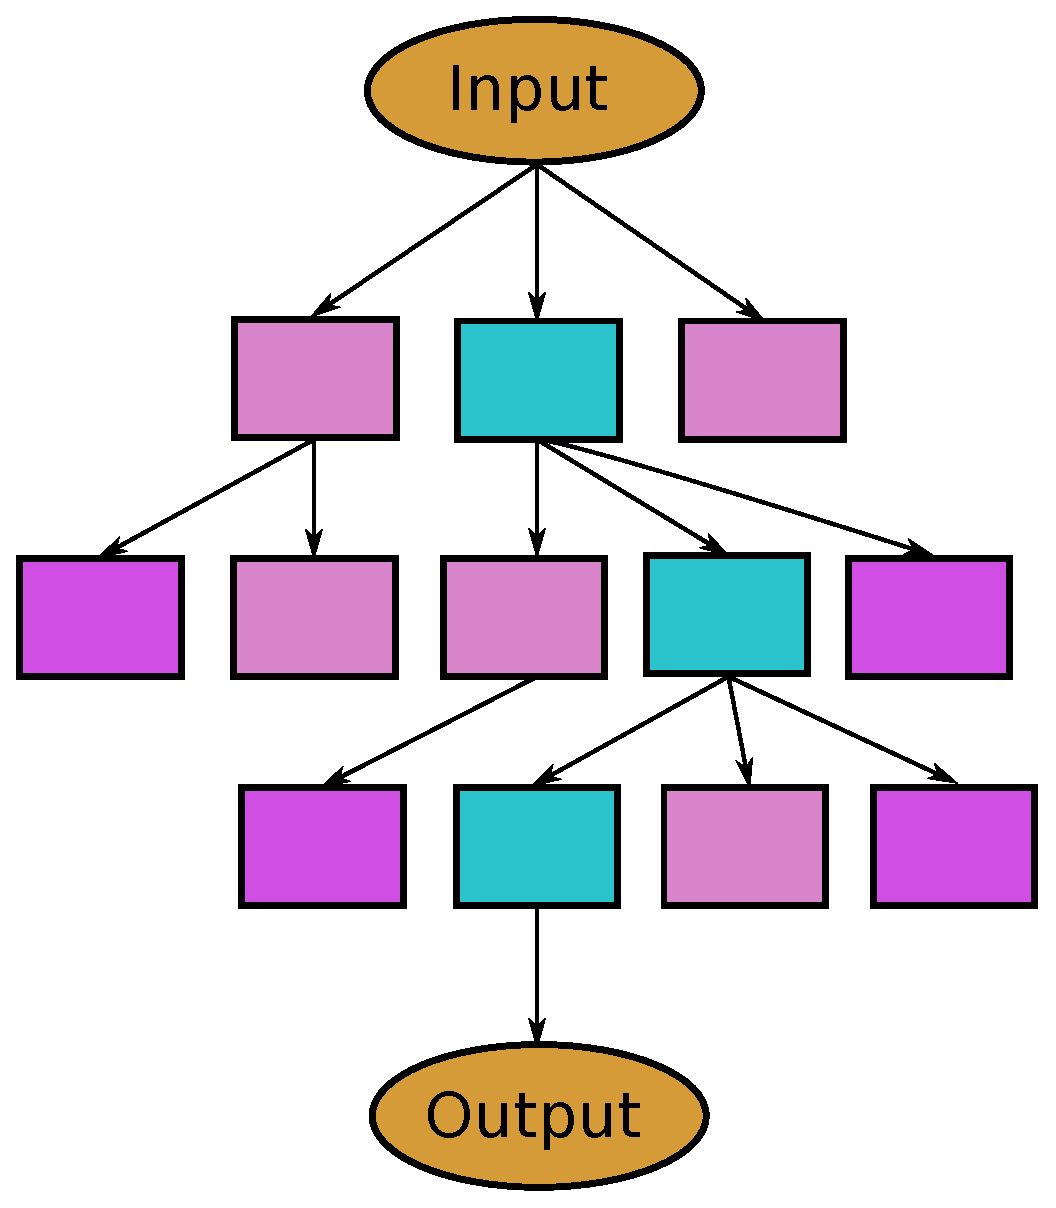
\includegraphics[width=0.4\textwidth]{content/chapter_basics/images/tot_schema.eps}
	\centering
	\caption{Baumstruktur der \glqq Tree of Thoughts\grqq \ Technik}
	\label{img:tot_schema}
\end{figure}

Im Folgenden ein Beispiel einer Teilaufgabe, bei der drei mögliche Lösungsvorschläge vom Modell erstellt wurden. Die Listings \ref{code:tot_php_dompdf}, \ref{code:tot_php_mpdf} und \ref{code:tot_php_tcpdf} zeigen die Ergebnisse des Modells. Es wurden jeweils andere PHP Bibliotheken für die Lösung vorgeschlagen. Als Modell wurde \textit{deepseek-coder-v2} verwendet. Als Nutzereingabe wurde folgendes an das Modell übergeben,

\epigraph{Erstelle drei verschiedene Methoden in PHP, die eine HTML Zeichenkette in ein PDF umwandeln und es als Datei, mit angegebenen Namen speichern.}

Die erste Lösung beinhaltet die Bibliothek \textit{Dompdf}.

\lstinputlisting[label={code:tot_php_dompdf},caption={Ausgabe für DOMPDF Bibliothek},language=PHP]{content/chapter_basics/codes/dompdf.php}

\lstinputlisting[label={code:tot_php_mpdf},caption={Ausgabe für MPDF Bibliothek},language=PHP]{content/chapter_basics/codes/mpdf.php}

Als dritte Ausgabe liefert coder,

\lstinputlisting[label={code:tot_php_tcpdf},caption={Ausgabe für TCPDF Bibliothek},language=PHP]{content/chapter_basics/codes/tcpdf.php}

%\subsubsection{Retrieval Augmented Generation}

%\subsubsection{Automatic Prompt Engineer}

%\subsubsection{Directional Stimulus Prompting}

%\subsubsection{ReAct}

%\subsubsection{Multimodal CoT}

%\subsubsection{Automatic Reasoning and Tool-use}

%\subsubsection{Active-Prompt}

%\subsubsection{Program-Aided Language Models}

%\subsubsection{Reflexion}

%\subsubsection{Graph Prompting}


\subsection{Grenzen beim Prompt-Engineering für LLMs}
Trotz der bemerkenswerten linguistischen Leistung, stoßen große Sprachmodelle an ihre Grenzen, unter anderem wie in \cite{amatriain-2024} beschrieben,

%\section{Relevante Arbeiten}
%In \cite{zhou-2022} wird der Prompt-Optimierungsprozess als Black-Box interpretiert. Der mit minimalen Eingaben ein menschenähnliches Niveau erreichen soll.

%----------------------------------------------------------------


\section{Grundlagen bei der Entwicklung von Webanwendungen}
Webanwendung
